\section{Project 7 - Transform Image Compression}
\subsection{Project Proposal}
There are two parts in this project. Both parts use \emph{lenna.tif} as test image.\\
\textbf{(a)} Investigate image compression based on DCT block transform coding on blocks of size 8x8. Compress the test image to different qualities by discarding some DCT coefficients based on zonal mask and threshold mask and using the inverse discrete cosine transform with fewer transform coefficients. Display the original, reconstructed and difference images. \\
\textbf{(b)} Investigate image compression based on wavelets. Consider four types of wavelets: Haar, Daubechies, Symlet and the biorthogonal Cohen-Daubechies-Feauveau. The corresponding parameters is given in problem set. Decompose the test image by wavelets to 3 levels, truncate the wavelet coefficient to 0 below some threshold. Reconstruct the image from the left coefficients. Display the wavelet transforms of the image, the reconstructed image and the difference image.

\subsection{Preliminaries}
\subsubsection{Block Transform Coding}
Block transform coding is a widely used technique appears in many compression standards (JPEG, M-JPEG, MPEG-1,2,4......). We divides an image into small non-overlapping blocks of equal size (e.g. $8\times 8$) and processes the blocks independently using a 2-D transform. A reversible linear transform is used to map each block into a set of transform coefficients, which are then quantized and coded. In this project, we use DCT as the transform function. The overview diagram of the block coding system is displayed in Fig.\ref{fig:blocksys}. 
\begin{figure}[h!]
	\centering	
	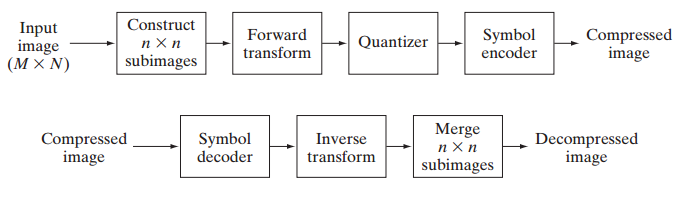
\includegraphics[width=0.4\linewidth]{myfigure/p7/block_system.png}
	\caption{Overview of block transform coding system with encoder and decoder.}
	\label{fig:blocksys}
\end{figure}
A forward discrete transform $T(u,v)$ of an $n\times n$ block can be expressed as \begin{equation} T(u,v)=\sum_{x=0}^{n-1}\sum_{y=0}^{n-1}g(x,y)r(x,y,u,v) \end{equation} and given $T(u,v)$, $g(x,y)$ can be obtained with inverse transform \begin{equation} g(x,y)=\sum_{u=0}^{n-1}\sum_{v=0}^{n-1}T(u,v)s(x,y,u,v) \end{equation} In these two equations, $r(x,y,u,v)$ and $s(x,y,u,v)$ are called \emph{forward} and \emph{inverse transformation kernels} respectively. They are also referred to basis functions or basis images. The $T(u,v)$ are called \emph{transform coefficients}.
\subsubsection{Discrete cosine transform (DCT)}
DCT is one of most frequently used image compression kernel
\begin{equation}\begin{aligned} r(x,y,u,v)&=s(x,y,u,v)\\ 
&=\alpha(u)\alpha(v)\cos\left[ \frac{(2x+1)u\pi}{2n}\right] \cos\left[ \frac{(2y+1)v\pi}{2n} \right]
\end{aligned}\end{equation} 
\begin{equation} \alpha(u) = \left\{ \begin{array}{rcl}
\sqrt{1/n} & \text{for } u=0 \\
\sqrt{2/n} & \text{for } u=1,2,...,n-1
\end{array} \right. \end{equation}
\subsubsection{Bit allocation}
Here we discuss two most popular methods for retained coefficients selection which is a masking function 
\begin{equation}\chi(u,v)= \left\{ \begin{array}{rcl}
0 & \text{if $T(u,v)$ satisfies a specified truncation criterion}\\
1 & \text{otherwise}
\end{array} \right. \end{equation}. One is based on maximum variance, called \emph{zonal coding} and the other is based on maximum magnitude called \emph{threshold coding}. The overall process of truncating, quantizing and coding the coefficients of transformed subimage is commonly called bit allocation. In Fig.\ref{fig:bitalloc} are typical forms of zonal mask and threshold mask. We construct zonal mask by placing a 1 in the locations of maximum variance and a 0 in all other locations. Coefficients of maximum variance usually are located around the origina of an image transform, resulting the typical zonal mask shown here. Threshold coding is adaptive in the sense that the location of the transform coefficients retained for each subimage vary from one subimage to another.\\
\begin{figure}[h!]
	\centering	
	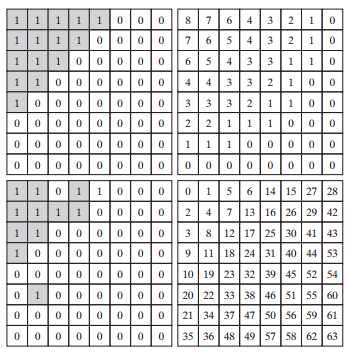
\includegraphics[width=0.7\linewidth]{myfigure/p7/bit_allocation.png}
	\caption{A typical (a)zonal mask, (b)zonal bit allocation, (c)threshold mask and (d)thresholded coefficient ordering sequence.}
	\label{fig:bitalloc}
\end{figure}

\subsection{Experiment}
The result of zonal mask and threshold mask compression using DCT transformation is displayed in Fig.\ref{fig:7dct}. I use two zonal masks. One is with 15 coefficients and the other is with 3 coefficients. The threshold mask is set to use median of the transform as the threshold. This is learned from the internet blog as I didn't find the threshold setting on the textbook.

\begin{figure}[h!]
	\centering
	\begin{subfigure}[b]{0.3\linewidth}
		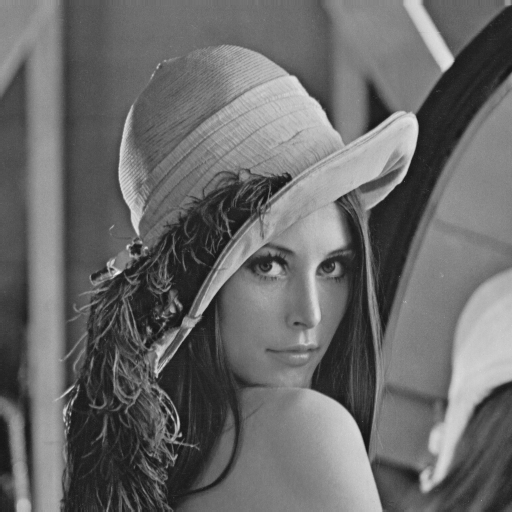
\includegraphics[width=\linewidth]{myfigure/p7/lenna.png}
		\caption{}
		\label{fig:lenna}
	\end{subfigure}
	\begin{subfigure}[b]{0.3\linewidth}
		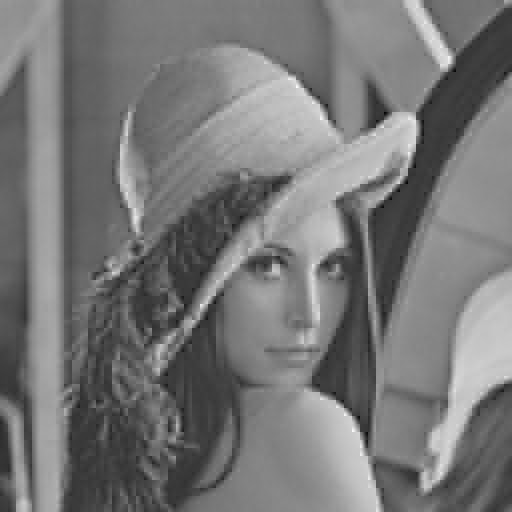
\includegraphics[width=\linewidth]{myfigure/p7/7_zonal_2.png}
		\caption{}
		\label{fig:7zonal2}
	\end{subfigure}
	\begin{subfigure}[b]{0.3\linewidth}
		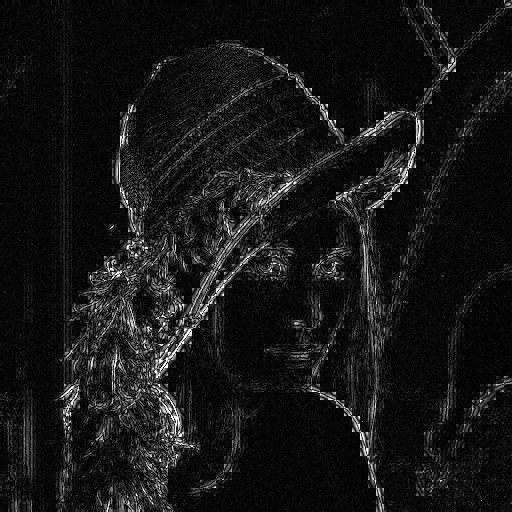
\includegraphics[width=\linewidth]{myfigure/p7/7_zonal_2_diff.png}
		\caption{}
		\label{fig:7zonal2diff}
	\end{subfigure}
	\begin{subfigure}[b]{0.3\linewidth}
		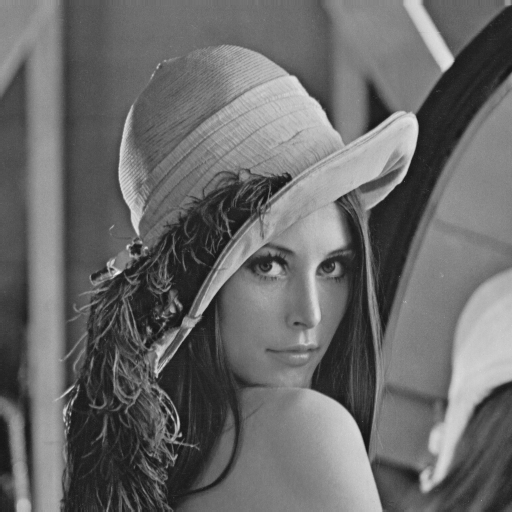
\includegraphics[width=\linewidth]{myfigure/p7/lenna.png}
		\caption{}
		\label{fig:lenna}
	\end{subfigure}
	\begin{subfigure}[b]{0.3\linewidth}
		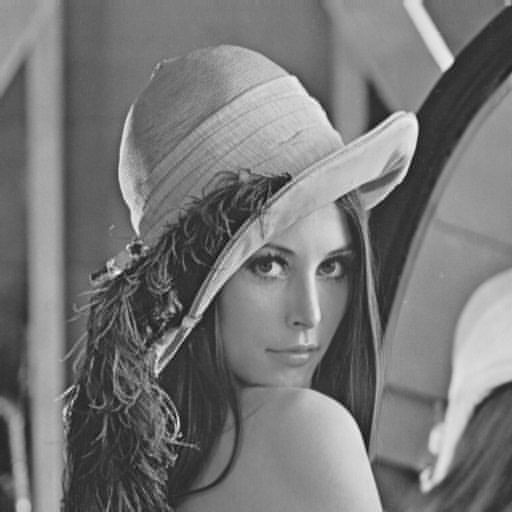
\includegraphics[width=\linewidth]{myfigure/p7/7_zonal_5.png}
		\caption{}
		\label{fig:7zonal5}
	\end{subfigure}
	\begin{subfigure}[b]{0.3\linewidth}
		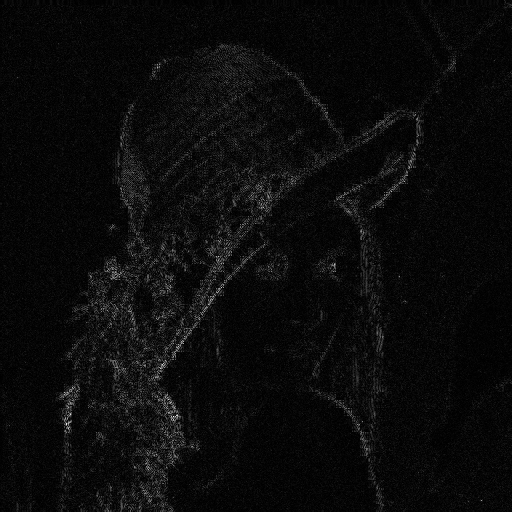
\includegraphics[width=\linewidth]{myfigure/p7/7_zonal_5_diff.png}
		\caption{}
		\label{fig:7zonal5diff}
	\end{subfigure}
	\begin{subfigure}[b]{0.3\linewidth}
		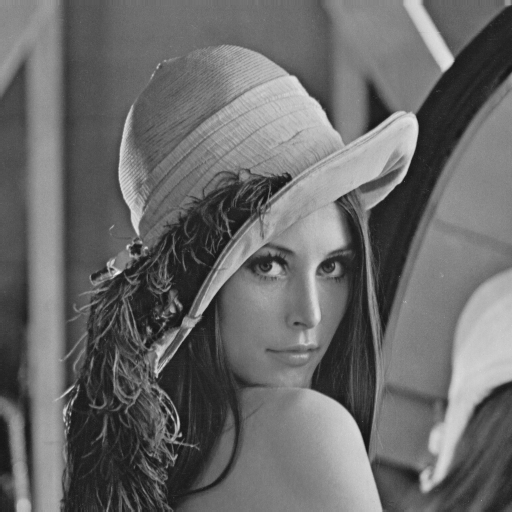
\includegraphics[width=\linewidth]{myfigure/p7/lenna.png}
		\caption{}
		\label{fig:lenna}
	\end{subfigure}
	\begin{subfigure}[b]{0.3\linewidth}
		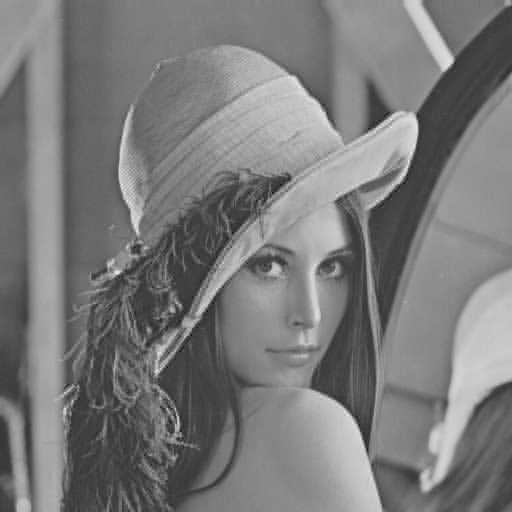
\includegraphics[width=\linewidth]{myfigure/p7/7_threshold_median.png}
		\caption{}
		\label{fig:7threshold}
	\end{subfigure}
	\begin{subfigure}[b]{0.3\linewidth}
		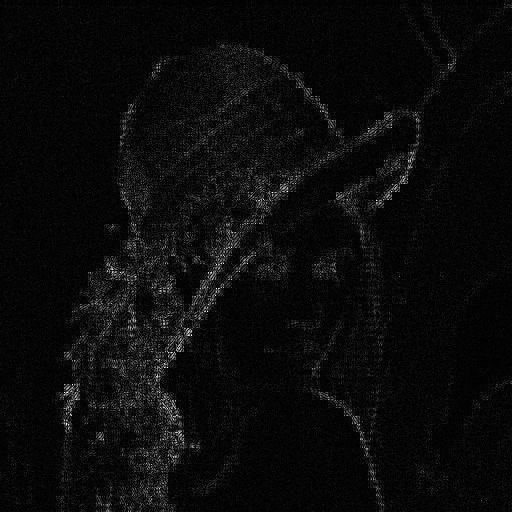
\includegraphics[width=\linewidth]{myfigure/p7/7_threshold_median_diff.png}
		\caption{}
		\label{fig:7thresholddiff}
	\end{subfigure}
	
	\caption{$8\times 8$ subimage DCT transform. First column are the same original image. Second column images are the compression result. The third column is the difference. \\1st Row: zonal mask with 15 coefficients. \\ 2nd Row: zonal mask with 3 coefficients. \\3rd Row: threshold mask using median value as threshold.}
	\label{fig:7dct}
\end{figure}

\clearpage
\subsection{Implementation}
The most important functions are \emph{dct\_mask, threshold\_coding, zonal\_coding}.
\lstset{language=Matlab}
\begin{lstlisting}
function [ dct_mask ] = dct_mask( n )
%DCT_MASK generate dct mask
%   m, n: the size of dct mask

dct_mask = zeros(n);
for u = (1:n)
    for x = (1:n)
        if u==1
            alphau = sqrt(1/n);
        else
            alphau = sqrt(2/n);
        end
        dct_mask(u,x) = alphau * cos(pi*(2*x-1)*(u-1)/2/n);
    end
end

end
\end{lstlisting}

\lstset{language=Matlab}
\begin{lstlisting}
function [ imgg, diff ] = zonal_coding( imgf, bsize, rx, ry, mask_num )
%ZONAL_CODING
%   bsize: size of subimage; rx, ry: transform mask; mask: zonal mask

[M, N] = size(imgf);
bm = fix(M/bsize);
bn = fix(N/bsize);
imgf = double(imgf);

% transform T
T = zeros(M, N);
for i = (1:bm)
    for j = (1:bn)
        xrange = (bsize*(i-1)+1 : bsize*i);
        yrange = (bsize*(j-1)+1 : bsize*j);
        T(xrange, yrange) = rx * imgf(xrange,yrange) * ry;
    end
end

% generate mask
mask = zeros(bsize, bsize);
for i = (1:bsize)
    for j = (1:bsize)
        if i+j<=mask_num+1
            mask(i,j) = 1;
        end
    end
end

% zonal mask
T_mask = zeros(M, N);
for i = (1:bm)
    for j = (1:bn)
        xrange = (bsize*(i-1)+1 : bsize*i);
        yrange = (bsize*(j-1)+1 : bsize*j);
        T_mask(xrange, yrange) = T(xrange,yrange) .* mask;
    end
end

% inverse transform
imgg = zeros(M, N);
for i = (1:bm)
    for j = (1:bn)
        xrange = (bsize*(i-1)+1 : bsize*i);
        yrange = (bsize*(j-1)+1 : bsize*j);
        imgg(xrange, yrange) = ry * T_mask(xrange,yrange) * rx;
    end
end

% calculcate difference
diff = abs(imgg - imgf);
diff = uint8(4*diff);

imgg = uint8(scale255(imgg));

end
\end{lstlisting}

\lstset{language=Matlab}
\begin{lstlisting}
function [ imgg, diff ] = threshold_coding( imgf, bsize, rx, ry )
%THRESHOLD_CODING 
%   bsize: size of subimage; rx, ry: transform mask;

[M, N] = size(imgf);
bm = fix(M/bsize);
bn = fix(N/bsize);
imgf = double(imgf);

% transform T
T = zeros(M, N);
for i = (1:bm)
    for j = (1:bn)
        xrange = (bsize*(i-1)+1 : bsize*i);
        yrange = (bsize*(j-1)+1 : bsize*j);
        T(xrange, yrange) = rx * imgf(xrange,yrange) * ry;
    end
end

% generate threshold 
mask = zeros(bsize, bsize);
med = median(rx(:));
for i = (1:bsize)
    for j = (1:bsize)
        if rx(i,j)>=med
            mask(i,j) = 1;
        end
    end
end

% threshold mask
T_mask = zeros(M, N);
for i = (1:bm)
    for j = (1:bn)
        xrange = (bsize*(i-1)+1 : bsize*i);
        yrange = (bsize*(j-1)+1 : bsize*j);
        T_mask(xrange, yrange) = T(xrange,yrange) .* mask;
    end
end

% inverse transform
imgg = zeros(M, N);
for i = (1:bm)
    for j = (1:bn)
        xrange = (bsize*(i-1)+1 : bsize*i);
        yrange = (bsize*(j-1)+1 : bsize*j);
        imgg(xrange, yrange) = ry * T_mask(xrange,yrange) * rx;
    end
end

% calculcate difference
diff = abs(imgg - imgf);
diff = uint8(4*diff);

imgg = uint8(scale255(imgg));

end
\end{lstlisting}



